\documentclass[t]{beamer}
\usetheme[english]{KIT}

\usepackage{amssymb} %% For \backprime
\usepackage{multicol}
\usepackage{mathpartir}

%\usepackage{mathpartir}
\usepackage{graphicx}

\usepackage{tikz}
\usetikzlibrary{arrows.meta,positioning,calc}

\usepackage[T1]{fontenc}
\usepackage{babel}
\usepackage{booktabs}
\usepackage[normalem]{ulem}
\usepackage{fontspec}
\setmonofont[RawFeature=-calt,Scale=MatchLowercase]{Iosevka}
%\newfontfamily\lc[Scale=MatchLowercase]{Iosevka SS09}

\usepackage{minted}
\definecolor{codebg}{rgb}{0.95,0.95,0.95}
\setminted{bgcolor=codebg,breaklines}
\usemintedstyle{tango}
\newmintinline[lean]{lean}{bgcolor=white}
\newminted[leancode]{theorem.py:LeanLexer -x}{fontsize=\footnotesize}

\usepackage{newunicodechar}
\newfontfamily{\freeserif}{DejaVu Sans}
\newunicodechar{ℕ}{\freeserif{ℕ}}
\newunicodechar{ℝ}{\freeserif{ℝ}}
\newunicodechar{ₐ}{\freeserif{ₐ}}
%\newunicodechar{₁}{\freeserif{₁}}
%\newunicodechar{∈}{\freeserif{∈}}
\newunicodechar{𝓞}{\ensuremath{\mathcal{O}}}
\newunicodechar{∉}{\freeserif{∉}}
%\newunicodechar{Π}{\freeserif{Π}}
%\newunicodechar{→}{\freeserif{→}}
\newunicodechar{⦃}{\freeserif{⦃}}
\newunicodechar{⦄}{\freeserif{⦄}}
%\newunicodechar{∧}{\freeserif{∧}}
%\newunicodechar{∨}{\freeserif{∨}}
%\newunicodechar{⊢}{\freeserif{⊢}}
\newunicodechar{⊑}{\freeserif{⊑}}
\newunicodechar{ₚ}{\freeserif{ₚ}}
\newunicodechar{∘}{\freeserif{∘}}
\newunicodechar{ₗ}{\freeserif{ₗ}}
\newunicodechar{∪}{\freeserif{∪}}
\newunicodechar{⋃}{\freeserif{⋃}}
\newunicodechar{𝓸}{\ensuremath{o}}
\newunicodechar{⊆}{\freeserif{⊆}}
\newunicodechar{≼}{\freeserif{≼}}
\newunicodechar{≃}{\freeserif{≃}}

% https://github.com/gpoore/minted/issues/220
\AtBeginEnvironment{snugshade*}{\vspace{-0.4\FrameSep}}
%\AfterEndEnvironment{snugshade*}{\vspace{-0.8\FrameSep}}

% https://tex.stackexchange.com/questions/343494/minted-red-box-around-greek-characters
\makeatletter
\AtBeginEnvironment{minted}{\dontdofcolorbox}
\def\dontdofcolorbox{\renewcommand\fcolorbox[4][]{##4}}
\makeatother

\title{Beyond Notations: Hygienic Macro Expansion for Theorem Proving Languages}

\author[Ullrich, de Moura]{\underline{Sebastian Ullrich}\inst{1}, Leonardo de Moura\inst{2}}
\subtitle{\insertauthor}
% \institute[IPD Snelting]{Programming paradigms group - IPD Snelting}
\institute[]{\inst{1}KIT, Germany\ \ \ \inst{2}Microsoft Research, USA}
\date{2020/07/01}
\makeatletter
\sbox{\KIT@titimg}{
  \hspace{0.08\titleimagewd}
    \raisebox{0.1\titleimageht}{
      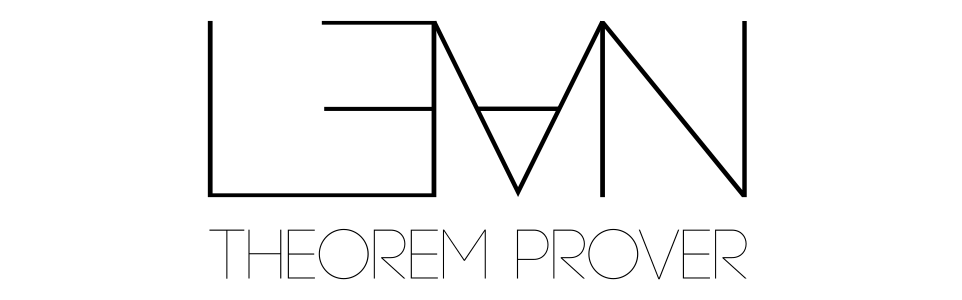
\includegraphics[height=0.8\titleimageht]{logo}
    }
}

\newcommand{\kit}[1]{\textcolor{KITgreen}{#1}}

\begin{document}
\begin{frame}
  \maketitle
\end{frame}

%\begin{frame}
%  \addtocounter{framenumber}{-1}
%  \maketitle
%\end{frame}

\begin{frame}{It's been a long time coming...}
  \vfill
  \fbox{
\includegraphics[width=\textwidth]{rfc}}
  \vfill
  \pause
  ``We should really refactor the elaborator as well''
  \vfill
  \pause
  ``If we rewrite the frontend, we should do that in Lean''
  \vfill
  \pause
  ``We first need a capable Lean compiler for that...''
  \vfill
  \pause
  Thus the Lean 4 project was born.
  \vfill
  \pause
  What issues could be that important?
\end{frame}

\begin{frame}[fragile]{Issues with existing syntax sugar systems}
  \begin{itemize}[<+->]
  \item Restricted to term level
    %\begin{onlyenv}<1>
\begin{leancode}
notation Γ `⊢` e `:` τ := Typing Γ e τ
\end{leancode}
    %\end{onlyenv}
  \item Restricted inputs
    %\begin{onlyenv}<2>
\begin{leancode}
notation `∃` binder `,` r:(scoped P, Exists P) := r
\end{leancode}
    \vspace{-0.5cm}
    \begin{onlyenv}<3>
\begin{leancode}
Notation "∃ x , P" := (exists (fun x => P)).
\end{leancode}
    \end{onlyenv}
    \begin{onlyenv}<4>
\begin{leancode}
Notation "\sum_ ( i <- r ) F"         := (\big[addn/0]_(i <- r) F).
Notation "\sum_ ( i <- r | P ) F"     := (\big[addn/0]_(i <- r | P) F).
Notation "\sum_ ( m <= i < n | P ) F" := (\big[addn/0]_(m <= i < n | P) F).
...
Notation "\mul_ ( i <- r ) F"         := (\big[muln/0]_(i <- r) F).
Notation "\mul_ ( i <- r | P ) F"     := (\big[muln/0]_(i <- r | P) F).
Notation "\mul_ ( m <= i < n | P ) F" := (\big[muln/0]_(m <= i < n | P) F).
...
\end{leancode}
      \vspace{-0.5cm}
    \end{onlyenv}
    \pause
    \pause
    %\end{onlyenv}
%  \item Restricted recursive syntax
%    \begin{onlyenv}<+>
%\begin{leancode}
%notation `[` l:(foldr `, ` (h t, List.cons h t) List.nil `]`) := l
%Notation "[ x ; .. ; y ]" := (cons x .. (cons y nil) ..).
%\end{leancode}
%    \end{onlyenv}
%    \pause
%    ...what I \emph{mean} is
%    \begin{onlyenv}<+>
%\begin{leancode}
%macro_rules
%| `([]) => `(List.nil)
%| `([$a, $a*]) => `(List.nil)
%\end{leancode}
%    \end{onlyenv}
  \item
    \begin{onlyenv}<5>
    Low-level might exist, but separate system!
\begin{leancode}
@[user_notation] meta def format_macro (_ : parse $ tk "format!") (s : string) :
  parser pexpr := ...
\end{leancode}
    \end{onlyenv}
  \end{itemize}
\end{frame}

\begin{frame}[fragile]{A unified frontend system}
  \pause
  \vspace{0.5cm}
  \begin{tabular}{clp{9cm}}
    Notations & \emph{Term} → \emph{Term} & \vspace{-0.45cm}
\begin{leancode}
notation "∃" b "," P => Exists (fun b => P)
\end{leancode}
    \\
    \pause
    $\Downarrow$ &&\\
    Macros & \emph{Surf} → \emph{Surf} & \vspace{-0.45cm}
\begin{leancode}
macro "∃" b:term "," P:term : term =>
`(Exists (fun $b => $P))
\end{leancode}
    \\
    \pause
    $\Downarrow$ &&\\
    Elaborators & \emph{Surf} → \emph{Core} & \vspace{-0.45cm}
\begin{leancode}
elab "∃" b:term "," P:term : term =>
`(Exists (fun $b => $P)) >>= elabTerm
\end{leancode}
  \end{tabular}
  \pause
  Equal hygiene guarantees for all levels
\end{frame}

\begin{frame}[fragile,fragile]{Hygiene}
\begin{leancode}
notation "const" e => fun x => e
\end{leancode}
  ``Of course'' $e$ may not capture $x$
  \pause
  \vfill
\begin{leancode}
macro "elab" ... => do
  ...;
  `(@[$elabAttr] def elabFn (stx : Syntax) : $type := match_syntax stx with ...)
\end{leancode}
  ``Of course'' \emph{elabFn} may not be captured from outside
  \pause
  \vfill
  $\Rightarrow$ Hygienic macros \underline{introduce scopes}!
\end{frame}

\begin{frame}[fragile]{Hygiene system}
  \begin{onlyenv}<1-2>
    Main inspiration: \emph{Binding as Sets of Scopes}, Matthew Flatt, POPL'16 \vfill
    \pause
    Streamlined \& optimized for slightly simpler macro system:\\
    no local macros, no mutual recursion between decls and macros
  \end{onlyenv}
  \pause
  In essence:
  \begin{enumerate}
  \item \emph{Remember} the surrounding scope in syntax quotations
\begin{leancode}
`(def elabFn{} (stx{} : Syntax{Lean.Syntax}) ...)
\end{leancode}
    \pause
  \item \emph{Tag} names introduced by macros
\begin{leancode}
def elabFn.23{} (stx.23{} : Syntax.23{Lean.Syntax}) ...
\end{leancode}
    (sequences of tags become important in macro-macros!)
  \end{enumerate}
  \vfill
  \pause
  Both actually implemented inside the \lean{`(...)} macro!
\end{frame}

\begin{frame}[fragile]{Adapted name resolution}
  \begin{enumerate}
  \item If tagged name is in local context, use it
\begin{leancode}
... (stx.23{} : ...) := match_syntax stx.23{} ...
\end{leancode}
    \kit{Implementation unchanged from basic name resolution}
    \pause
    \vfill
  \item Otherwise, check global scopes \kit{and remembered names if any}
\begin{leancode}
Syntax.23{Lean.Syntax}
\end{leancode}
  \pause
  \vfill
  \item Otherwise fail
  \end{enumerate}
  \vfill
\end{frame}

\begin{frame}[fragile]{Examples: Lean 4 elaborator}
  \pause
\begin{leancode}
syntax "if" optIdent term "then" term "else" term : term
macro_rules
| `(if $h : $cond then $t else $e) => `(dite $cond (fun $h => $t) (fun $h => $e))
| `(if $cond then $t else $e)      => `(ite $cond $t $e)
\end{leancode}
\end{frame}
\begin{frame}[fragile]{Examples: Lean 4 elaborator}
\[term ::= ... | \langle term, ..., term \rangle\]
\pause
\[\inferrule{
    \Gamma \vdash \tau \equiv I\ \overline{p} \\
    c\text{ is single constructor of }I \\
    \Gamma \vdash c\ \overline{t} \Leftarrow \tau \rightsquigarrow t' \\
  }{\Gamma \vdash \langle \overline{t} \rangle \Leftarrow \tau \rightsquigarrow t'}\]
\pause
\only<3>{\setminted{highlightlines=1}}
\only<4>{\setminted{highlightlines=2}}
\only<5>{\setminted{highlightlines=3-4}}
\only<6>{\setminted{highlightlines=5-7}}
\only<7>{\setminted{highlightlines=8-9}}
\begin{leancode}
elab "⟨" args:(sepBy term ", ") "⟩" : term <= τ => do
  τ ← whnf τ;
  match τ.getAppFn with
  | Expr.const I _ _ => do
    ctors ← getCtors I;
    match ctors with
    | [c] => do
      stx ← `($(mkCTermId c) $(getSepElems args.getArgs)*);
      elabTerm stx τ
  ... -- error handling
\end{leancode}
\end{frame}

\begin{frame}[fragile]{Examples: simple web server}
\only<2>{\setminted{highlightlines=5-8}}
\begin{leancode}
import Webserver

GET / => redirect "/greet/stranger"

GET /greet/{name} => write
  <html>
    <h1>Hello, {name}!</h1>
  </html>

def main : IO Unit := do
  hIn ← IO.stdin;
  hOut ← IO.stdout;
  Webserver.run hIn hOut
\end{leancode}

\url{https://leanprover.github.io/talks/PLDI20}

\end{frame}

\begin{frame}[fragile,fragile]{Tactic Hygiene}
  Lean 3 helper for proving injectivity of constructors:
\begin{leancode}
def mk_inj_eq : tactic unit :=
`[intros, apply propext, apply iff.intro, ...]
\end{leancode}
  Passable because no-one would ever redefine \lean{iff.intro}... right?
  \vfill
  \pause
\begin{leancode}
namespace hott
...
@[hott] def iff.intro : ...
...
inductive ... -- breaks!
\end{leancode}
  \pause
  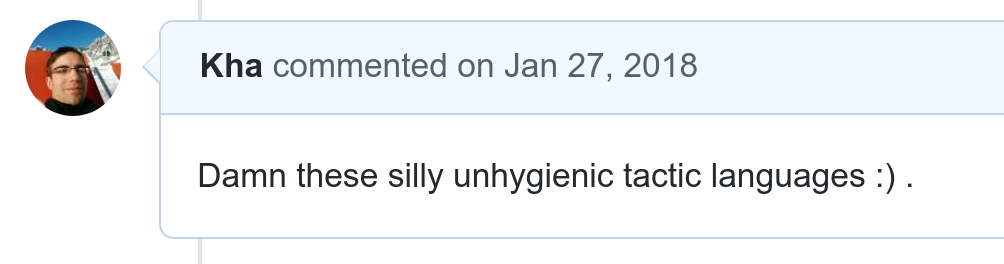
\includegraphics[width=0.6\textwidth]{damn.png}
\end{frame}

\begin{frame}[fragile]{Tactic Hygiene}
  Lean 4:
\begin{leancode}
macro mkInjEq : tactic =>
`(intros; apply propext; apply Iff.intro; ...)
\end{leancode}
  Tactic macros expanded on the fly by a new \kit{tactic interpreter}

  Same hygiene guarantees as with other macros
  \pause
  \vfill
\begin{leancode}
macro introH : tactic => `(intro h)
lemma ... by introH; exact h  -- breaks!
\end{leancode}
  \pause
\begin{leancode}
macro introH : tactic => `(intro $(mkIdent `h))
lemma ... by introH; exact h  -- works!
\end{leancode}
  %Hygiene is opt-out inside quotations, opt-in outside
\end{frame}

\begin{frame}{Conclusion}
  \begin{itemize}
  \item A tower of abstractions from notations down to elaborators
  \item A simple, non-invasive but effective macro hygiene system
  \item The first hygienic tactic system of its kind
  \end{itemize}
  \vfill
  \pause
  \begin{center}
    \Huge{Thank you!}
  \end{center}
\end{frame}
\end{document}

%%% Local Variables:
%%% mode: latex
%%% TeX-master: t
%%% TeX-engine: xetex
%%% TeX-command-extra-options: "-shell-escape"
%%% End:
